% !Mode:: "TeX:UTF-8"

\chapter{图计算相关概念与技术}

\section{图的相关概念}
图是一种复杂的抽象数据结构,能够表示不同物件之间的关系\cite{sunhuiquan2004}。
%而现实世界的数据量又非常巨大,常规的处理方法难以满足要求,因此需要进行大规模的图计算的研究。
从数据结构的角度出发,图是由有穷非空的顶点集合和表示顶点之间关系的边的集合组成。假如我们使用$G$表示一个图,$V$是图中顶点的集合,$E$表示是图中边的集合,那么一个图就可以表示为:$G=(V,E)$。
在图中,若顶点$Vi$到$Vj$的边没有方向,则这条边是无向边,无向边可以使用无序二元组$(V_i,V_j)$表示。如果图中任意两个顶点之间的边都是无向边,则该图是无向图,而一个图的任意两个顶点之间都有一条边,则称该图为无向完全图;若顶点$V_i$到$V_j$的边有方向,则称这条边为有向边,有向边可以使用有序二元组$(V_i,V_j)$表示,其中$V_i$表示起始顶点,$V_j$称为目的顶点。如果图中任意两个顶点之间的边都是有向边,则称该图为有向图,而有向图中任意两个顶点间都有方向相反的两条有向边,则该有向图为有向完全图。含有n个顶点的无向完全图有$n(n-1)/2$条边,含有n个顶点的有向完全图有$n(n-1)$条边。

在无向图中,一个顶点拥有的边的数量就是该顶点的度。在有向图中,顶点的出度就是以该顶点为起始顶点的边的数量,顶点的入度就是以该顶点为目的顶点的边的数目,该顶点的度为它自身入度和出度之和。在图的边上对其进行标示数字来标示该边的相关的数据信息,则该信息称为边的权重。边上带有权重的图就称为网。

在图中,若存在一系列首尾相接的边组成的顶点序列($V_i$,$V_m$,$V_n$,......,$V_j$)使得从顶点$V_i$到达顶点$V_j$,则称该序列为顶点$V_i$到顶点$V_j$的路径。其中,路径上边的数目就是该路径的长度,若是带权图,则路径的长度是该路径上边的权重之和。若一条路径的起始顶点和终止顶点相同,则称该路径为回路。若路径中只有起始顶点和终止定点是同一定点的路径称为简单回路。否则,没有相同顶点的路径称为简单路径。

如果图$G^0$的顶点和边属于图$G$则称图$G^0$是$G$的子图。在无向图中,如果存在一条从顶点$V_i$到顶点$V_j$的路径,则称顶点$V_i$到顶点$V_j$是连通的。若图中的任意两个顶点都是连通的则称该图为连通图。


\section{常见图算法}
图论作为数学领域中的一个重要分支已经有数百年的历史。人们发现图的许多重要特性,发明了许多重要的算法,其中许多困难问题的研究仍然十分活跃。在解决现实问题时,其他数据结构,例如线性表、树等,都具有明显的条件限制,而图结构中任意两个数据元素间均可相关联。在结构和语义方面,图较之线性表和树更为复杂,但是也更加具有表现能力。因此,现实世界中的数据往往都是以图的结构进行保存。

\subsection{图的存储}
在计算机中,要表示一个图$G=(V,E)$,有两种标准的方法:邻接矩阵和邻接表。这两种方法既可以表示有向图,也可以用来表示无向图。
邻接表表示由一个顶点$V$和以该顶点为起始顶点的边的集合组成。对于图$G$中每个顶点$V$$_i$,把所有邻接于顶点$V$$_i$的顶点$V$$_j$保持为一个单链表,则该单链表称为顶点$V$$_i$的邻接表,如图\ref{fig:graphdemo:adj}所示。邻接矩阵表示的原理就是利用两个数组,其中一个数组用来保存顶点,另外一个数组用来表示边,矩阵中为1的位置表示存在一条边,否则为0,如图\ref{fig:graphdemo:matrix}所示。

另外,图还可以用CSR(Compressed Sparse Row)格式进行保存,CSR格式将顶点\textit{id}和边分别用两个数组进行保存,其中边数组保存边的目的顶点\textit{id}并按照出发顶点\textit{id}排序就,而在顶点数组中顶点的\textit{id}就是数组的索引,每个顶点保存第一条边在在边数组中的索引,如图\ref{fig:graphdemo:csr}所示。
\begin{figure}[htbp]
  \centering
  \subfigure[5个顶点的无向图]{
            \label{ fig:graphdemo:demo)}
            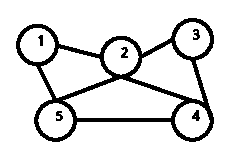
\includegraphics[width=0.2\textwidth]{myfigures/graphdemo.eps}}
  \subfigure[邻接表表示]{
            \label{fig:graphdemo:adj}
            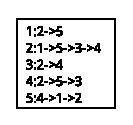
\includegraphics[width=0.15\textwidth,scale=0.5]{myfigures/graphadj.eps}}
  \subfigure[邻接矩阵表示]{
            \label{fig:graphdemo:matrix}
            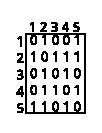
\includegraphics[width=0.1\textwidth,scale=0.5]{myfigures/graphmatrix.eps}}
\subfigure[CSR表示]{
            \label{fig:graphdemo:csr}
            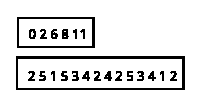
\includegraphics[width=0.2\textwidth]{myfigures/graphcsr.eps}}
  \caption{图的表示方法}\label{fig:graphdemo}
\vspace{\baselineskip}
\end{figure}

\subsection{遍历图}
图的遍历是指从图中给定的某一源点出发,对图中的顶点访问且近且访问一次的操作。图的遍历算法有两种:广度优先和深度优先。

广度优先搜索是最简单的图算法之一,也是很多其他图算法的重要基础。对于给定的图$G=(V,E)$和一个确定的源顶点$s$,广度搜索算法的主要流程如下:
\begin{itemize}
\item 首先访问顶点$s$,并将顶点$s$标记为已访问。
\item 依次搜索$s_0$所有邻接顶点$s_1$,$s_2$,...,$s_m$,并将其标记为已访问。
\item 再按照$s_1$,$s_2$,...,$s_m$的次序依次访问它们的未被访问过的邻接顶点,并将其标记为已访问
\item 以此类推,直到图中所有和源顶点$s_0$有路径相同的顶点都被访问过为止,如图\ref{fig:graphbfs}所示。
\end{itemize}

\begin{figure}[htbp]
\centering
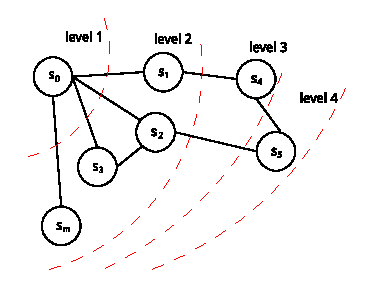
\includegraphics[width=0.4\textwidth]{myfigures/graphbfs}
\caption{广度优先遍历}\label{fig:graphbfs}
\vspace{\baselineskip}
\end{figure}

对于给定的图$G=(V,E)$和一个确定的源顶点$s$,深度优先遍历的基本流程如下:
\begin{itemize}
\item 首先访问顶点$s$,并将顶点$s$标记为已访问。
\item 依次搜索$s_0$的所有邻接顶点$s_i$,若$s_i$没有被访问过,则把顶点$s_i$作为新的源点,继续深度优先遍历,知道图中所有和顶点$s_0$有路径的顶点都被访问一次为止。
\item 如果图中存其他未被访问的顶点,则另选一个作为源点,重复上述步骤,直到所有顶点都被访问过为止,如图\ref{fig:graphdfs}所示。
\end{itemize}

\begin{figure}[htbp]
\centering
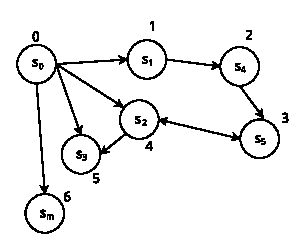
\includegraphics[width=0.4\textwidth]{myfigures/graphdfs}
\caption{深度优先遍历}\label{fig:graphdfs}
\vspace{\baselineskip}
\end{figure}

\subsection{单源最短路径}
单源最短路径是图论中寻找从开始顶点到某一终止顶点的的最短的路径算法。对于已知图$G=(V,E)$,寻找从给定的源点$s$到顶点$S_i ∈ V$ 的最短路径。最常见的算法就是Dijkstra算法,它的主要思想是:如果路径$P$是从源点$s_0$到顶点$s_j$的最短路径,其中顶点$s_i$是路径中的一个点,则从顶点$s_0$沿着路径$P$到顶点$s_i$的路径就是从顶点$s_0$到顶点$s_i$的最短路径。假设源点为$s_0$,集合$U={s_0}$,distance[i]记录从顶点$s_0$到顶点$s_i$的最短路径,path[i]记录从顶点$s_0$到顶点$s_i$的路径上的前一个顶点,则Dijkstra算法的主要流程如下:

\begin{itemize}
\item 从顶点集合$V-U$中选择使distance[i]最小的顶点$s_i$,并将顶点$s_i$加入集合$U$。
\item 更新与顶点$s_i$直接相邻的distance值。
\item 重复以上步骤,直到顶点集合$U$与图的顶点集合$V$相同,则计算完成。
\end{itemize}


\subsection{最小生成树}
最小生成树是指用少的边连接图中所有的顶点。最常见的最小生成树算法是Prime算法和kruskal算法。Prime算法的主要思想是从某一顶点开始,选择与它相邻的具有最小权重的边,并将该顶点加入到生成的树的顶点集合中,然后每一步都从一个顶点在生成树的顶点集中而另一个顶点不在该集合的各条边中选择权重最小的边,并将顶点加入生成树的顶点集合中。如此往复,直到图中的所有顶点都加入到生成树中为止,如图\ref{fig:prime}所示。假设无向带权连通图$G=(V,E)$,$T=(U,ET)$是最小生成树,其中$U$是最小生成树的顶点的集合,$ET$是最小生成树的边的集合,则Prime的算法流程:

\begin{itemize}
\item 初始化,$ET$为空,$U={s_0}$。
\item 对于所有边$(s_i,s_j)$,其中顶点$s_i$属于最小生成树的顶点集合$U$,顶点$s_j$不属于最小生成树的顶点集合$U$,选择权重最小的一条边加入最小生成树。
\item 重复步骤2,直到所有顶点都加入最小生成树中。
\end{itemize}


\begin{figure}[htbp]
\centering
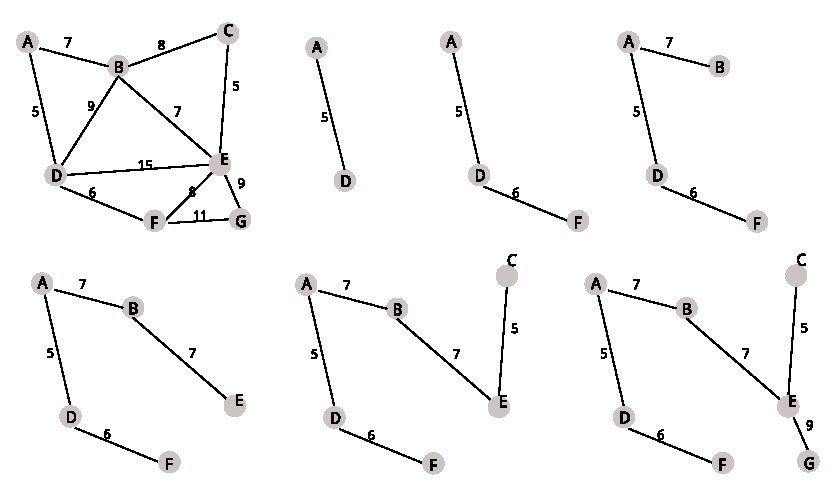
\includegraphics[width=0.6\textwidth]{myfigures/prime}
\caption{Prime算法示例}\label{fig:prime}
\vspace{\baselineskip}
\end{figure}

kruskal算法的主要思想是将图的n个顶点看做是一个含有n棵树的森林,然后从图中选择一条权值最小的边,如果该边的两个顶点属于两个不同的树,则将两个树合成一棵树,否则如果该边的两个顶点已经属于同一棵树,则不可取,一次类推,直至森林中只有一棵树为止,如图\ref{fig:kruskal}所示。假设无向带权连通图$G=(V,E)$,$T=(U,ET)$是最小生成树,其中$U$是最小生成树的顶点的集合,$ET$是最小生成树的边的集合,则kruskal的算法流程:
\begin{itemize}
\item 初始化,n棵树的森林
\item 对于所有边$(s_i,s_j)$,选择权值最小的边,如果顶点$s_i$和$s_j$属于两棵不同的树则加入,否则不可取。
\item 重复步骤2,直到森林中只剩下一棵树。
\end{itemize}

\begin{figure}[htbp]
\centering
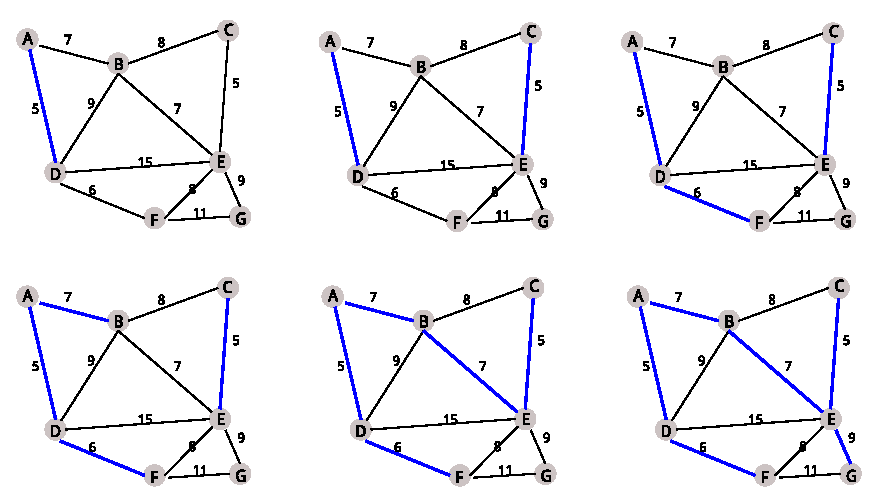
\includegraphics[width=0.6\textwidth]{myfigures/kruskal}
\caption{kruskal算法示例}\label{fig:kruskal}
\vspace{\baselineskip}
\end{figure}

\subsection{PageRank}

PageRank是著名的网页排名算法。PageRank是一种根据网页之间的相互连接的投票关系对网页在网络中所占的权重进行计算的一种算法。在网络世界中,网页之间通过超链接互相联系,如果把网页看做顶点,网页之间的超链接关系看做是边,整个网络都可以看成一个图。通过对各个网页在网络中的权重进行计,有利于提高搜索结果的准确性和相关性。在PageRank中,如果网页$Page_i$存在一条指向网页$Page_j$的一个超链接,那么就说网页$Page_i$给网页$Page_j$投票。一般来说,权重的网页所指向的网页也往往是权重比较重的网页,同样的高权重的网页指向一个低权重的网页,也可以使低权重的网页的权重提升。其中每个网页的初始权重为1/n,那么该网页每有一个连接指向其他网页,那么该网页对其他网页提供的投票数为1,若有n个链接指向其他网页,那么该网页对其他网页每个提供1/n的投票。反之,如果某个网页收到来自其他网页的投票数之和即为该网页自身的权重。如上所示,进行多次迭代,直到所有网页的权重都趋于收敛则计算结束。

\begin{figure}[htbp]
\centering
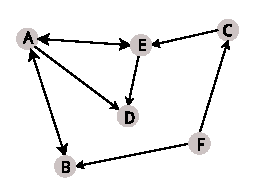
\includegraphics[width=0.4\textwidth]{myfigures/pagerank}
\caption{kruskal算法示例}\label{fig:pagerank}
\vspace{\baselineskip}
\end{figure}

如图\ref{fig:pagerank}所示,一个由5个网页组成的网图关系,A分别给网页B、网页D、网页E提供权重为1/3的投票,B给网页A提供权重为1的投票,C给网页E提供权重为1的投票,D由于没有玩连接所以D默认给每个网页提供权重为1/6的投票,E分别给网页提供群众为1/2的投票,F分别给网页提供权重为1/2的投票,构造的投票的矩阵$h$如下所示:
% MathType!MTEF!2!1!+-
% feaagKart1ev2aaatCvAUfeBSjuyZL2yd9gzLbvyNv2CaerbuLwBLn
% hiov2DGi1BTfMBaeXatLxBI9gBaerbd9wDYLwzYbItLDharqqtubsr
% 4rNCHbGeaGqiVu0Je9sqqrpepC0xbbL8F4rqqrFfpeea0xe9Lq-Jc9
% vqaqpepm0xbba9pwe9Q8fs0-yqaqpepae9pg0FirpepeKkFr0xfr-x
% fr-xb9adbaqaaeGaciGaaiaabeqaamaabaabaaGcbaGaamiAaiabg2
% da9maadmaabaqbaeqabCWbaaaaaeaaaeaacaWGbbaabaGaamOqaaqa
% aiaadoeaaeaacaWGebaabaGaamyraaqaaiaadAeaaeaacaWGbbaaba
% GaaGimaaqaaiaaicdaaeaacaaIWaaabaGaaGimaaqaamaaliaabaGa
% aGymaaqaaiaaikdaaaaabaGaaGimaaqaaiaadkeaaeaadaWccaqaai
% aaigdaaeaacaaIZaaaaaqaaiaaicdaaeaacaaIWaaabaGaaGimaaqa
% aiaaicdaaeaadaWccaqaaiaaigdaaeaacaaIYaaaaaqaaiaadoeaae
% aacaaIWaaabaGaaGimaaqaaiaaicdaaeaacaaIWaaabaGaaGimaaqa
% amaaliaabaGaaGymaaqaaiaaikdaaaaabaGaamiraaqaamaaliaaba
% GaaGymaaqaaiaaiodaaaaabaGaaGimaaqaaiaaicdaaeaacaaIWaaa
% baWaaSGaaeaacaaIXaaabaGaaGOmaaaaaeaacaaIWaaabaGaamyraa
% qaamaaliaabaGaaGymaaqaaiaaiodaaaaabaGaaGimaaqaaiaaigda
% aeaacaaIWaaabaGaaGimaaqaaiaaicdaaeaacaWGgbaabaGaaGimaa
% qaaiaaicdaaeaacaaIWaaabaGaaGimaaqaaiaaicdaaeaacaaIWaaa
% aaGaay5waiaaw2faaiabgUcaRmaadmaabaqbaeqabCWbaaaaaeaaae
% aacaWGbbaabaGaamOqaaqaaiaadoeaaeaacaWGebaabaGaamyraaqa
% aiaadAeaaeaacaWGbbaabaGaaGimaaqaamaaliaabaGaaGymaaqaai
% aaiAdaaaaabaGaaGimaaqaamaaliaabaGaaGymaaqaaiaaiAdaaaaa
% baGaaGimaaqaaiaaicdaaeaacaWGcbaabaGaaGimaaqaamaaliaaba
% GaaGymaaqaaiaaiAdaaaaabaGaaGimaaqaamaaliaabaGaaGymaaqa
% aiaaiAdaaaaabaGaaGimaaqaaiaaicdaaeaacaWGdbaabaGaaGimaa
% qaamaaliaabaGaaGymaaqaaiaaiAdaaaaabaGaaGimaaqaamaaliaa
% baGaaGymaaqaaiaaiAdaaaaabaGaaGimaaqaaiaaicdaaeaacaWGeb
% aabaGaaGimaaqaamaaliaabaGaaGymaaqaaiaaiAdaaaaabaGaaGim
% aaqaamaaliaabaGaaGymaaqaaiaaiAdaaaaabaGaaGimaaqaaiaaic
% daaeaacaWGfbaabaGaaGimaaqaamaaliaabaGaaGymaaqaaiaaiAda
% aaaabaGaaGimaaqaamaaliaabaGaaGymaaqaaiaaiAdaaaaabaGaaG
% imaaqaaiaaicdaaeaacaWGgbaabaGaaGimaaqaamaaliaabaGaaGym
% aaqaaiaaiAdaaaaabaGaaGimaaqaamaaliaabaGaaGymaaqaaiaaiA
% daaaaabaGaaGimaaqaaiaaicdaaaaacaGLBbGaayzxaaaaaa!93EA!
\[h = \left[ {\begin{array}{*{20}{c}}
{}&A&B&C&D&E&F\\
A&0&0&0&0&{{\raise0.7ex\hbox{$1$} \!\mathord{\left/
 {\vphantom {1 2}}\right.\kern-\nulldelimiterspace}
\!\lower0.7ex\hbox{$2$}}}&0\\
B&{{\raise0.7ex\hbox{$1$} \!\mathord{\left/
 {\vphantom {1 3}}\right.\kern-\nulldelimiterspace}
\!\lower0.7ex\hbox{$3$}}}&0&0&0&0&{{\raise0.7ex\hbox{$1$} \!\mathord{\left/
 {\vphantom {1 2}}\right.\kern-\nulldelimiterspace}
\!\lower0.7ex\hbox{$2$}}}\\
C&0&0&0&0&0&{{\raise0.7ex\hbox{$1$} \!\mathord{\left/
 {\vphantom {1 2}}\right.\kern-\nulldelimiterspace}
\!\lower0.7ex\hbox{$2$}}}\\
D&{{\raise0.7ex\hbox{$1$} \!\mathord{\left/
 {\vphantom {1 3}}\right.\kern-\nulldelimiterspace}
\!\lower0.7ex\hbox{$3$}}}&0&0&0&{{\raise0.7ex\hbox{$1$} \!\mathord{\left/
 {\vphantom {1 2}}\right.\kern-\nulldelimiterspace}
\!\lower0.7ex\hbox{$2$}}}&0\\
E&{{\raise0.7ex\hbox{$1$} \!\mathord{\left/
 {\vphantom {1 3}}\right.\kern-\nulldelimiterspace}
\!\lower0.7ex\hbox{$3$}}}&0&1&0&0&0\\
F&0&0&0&0&0&0
\end{array}} \right] + \left[ {\begin{array}{*{20}{c}}
{}&A&B&C&D&E&F\\
A&0&{{\raise0.7ex\hbox{$1$} \!\mathord{\left/
 {\vphantom {1 6}}\right.\kern-\nulldelimiterspace}
\!\lower0.7ex\hbox{$6$}}}&0&{{\raise0.7ex\hbox{$1$} \!\mathord{\left/
 {\vphantom {1 6}}\right.\kern-\nulldelimiterspace}
\!\lower0.7ex\hbox{$6$}}}&0&0\\
B&0&{{\raise0.7ex\hbox{$1$} \!\mathord{\left/
 {\vphantom {1 6}}\right.\kern-\nulldelimiterspace}
\!\lower0.7ex\hbox{$6$}}}&0&{{\raise0.7ex\hbox{$1$} \!\mathord{\left/
 {\vphantom {1 6}}\right.\kern-\nulldelimiterspace}
\!\lower0.7ex\hbox{$6$}}}&0&0\\
C&0&{{\raise0.7ex\hbox{$1$} \!\mathord{\left/
 {\vphantom {1 6}}\right.\kern-\nulldelimiterspace}
\!\lower0.7ex\hbox{$6$}}}&0&{{\raise0.7ex\hbox{$1$} \!\mathord{\left/
 {\vphantom {1 6}}\right.\kern-\nulldelimiterspace}
\!\lower0.7ex\hbox{$6$}}}&0&0\\
D&0&{{\raise0.7ex\hbox{$1$} \!\mathord{\left/
 {\vphantom {1 6}}\right.\kern-\nulldelimiterspace}
\!\lower0.7ex\hbox{$6$}}}&0&{{\raise0.7ex\hbox{$1$} \!\mathord{\left/
 {\vphantom {1 6}}\right.\kern-\nulldelimiterspace}
\!\lower0.7ex\hbox{$6$}}}&0&0\\
E&0&{{\raise0.7ex\hbox{$1$} \!\mathord{\left/
 {\vphantom {1 6}}\right.\kern-\nulldelimiterspace}
\!\lower0.7ex\hbox{$6$}}}&0&{{\raise0.7ex\hbox{$1$} \!\mathord{\left/
 {\vphantom {1 6}}\right.\kern-\nulldelimiterspace}
\!\lower0.7ex\hbox{$6$}}}&0&0\\
F&0&{{\raise0.7ex\hbox{$1$} \!\mathord{\left/
 {\vphantom {1 6}}\right.\kern-\nulldelimiterspace}
\!\lower0.7ex\hbox{$6$}}}&0&{{\raise0.7ex\hbox{$1$} \!\mathord{\left/
 {\vphantom {1 6}}\right.\kern-\nulldelimiterspace}
\!\lower0.7ex\hbox{$6$}}}&0&0
\end{array}} \right]\]
为了能够确保PageRank能够快速收敛结束运算,在实际进行计算时,往往需要让投票矩阵乘以一个阻尼系数,该阻尼系数一般为0.85,同时由于没有外链接的网页传递出去的权重会是0,所以需要给每个页面一个最小值,如下$G$所示:

% MathType!MTEF!2!1!+-
% feaagKart1ev2aaatCvAUfeBSjuyZL2yd9gzLbvyNv2CaerbuLwBLn
% hiov2DGi1BTfMBaeXatLxBI9gBaerbd9wDYLwzYbItLDharqqtubsr
% 4rNCHbGeaGqiVu0Je9sqqrpepC0xbbL8F4rqqrFfpeea0xe9Lq-Jc9
% vqaqpepm0xbba9pwe9Q8fs0-yqaqpepae9pg0FirpepeKkFr0xfr-x
% fr-xb9adbaqaaeGaciGaaiaabeqaamaabaabaaGcbaGaam4raiabg2
% da9iaaicdacaGGUaGaaGioaiaaiwdacaGGQaGaamiAaiabgUcaRmaa
% dmaabaqbaeqabCWbaaaaaeaaaeaacaWGbbaabaGaamOqaaqaaiaado
% eaaeaacaWGebaabaGaamyraaqaaiaadAeaaeaacaWGbbaabaGaaGym
% aaqaaiaaigdaaeaacaaIXaaabaGaaGymaaqaaiaaigdaaeaacaaIXa
% aabaGaamOqaaqaaiaaigdaaeaacaaIXaaabaGaaGymaaqaaiaaigda
% aeaacaaIXaaabaGaaGymaaqaaiaadoeaaeaacaaIXaaabaGaaGymaa
% qaaiaaigdaaeaacaaIXaaabaGaaGymaaqaaiaaigdaaeaacaWGebaa
% baGaaGymaaqaaiaaigdaaeaacaaIXaaabaGaaGymaaqaaiaaigdaae
% aacaaIXaaabaGaamyraaqaaiaaigdaaeaacaaIXaaabaGaaGymaaqa
% aiaaigdaaeaacaaIXaaabaGaaGymaaqaaiaadAeaaeaacaaIXaaaba
% GaaGymaaqaaiaaigdaaeaacaaIXaaabaGaaGymaaqaaiaaigdaaaaa
% caGLBbGaayzxaaGaaiOkamaalaaabaGaaGimaiaac6cacaaIXaGaaG
% ynaaqaaiaaiAdaaaGaeyypa0ZaamWaaeaafaqabeGbgaaaaaqaaiaa
% icdacaGGUaGaaGimaiaaiodaaeaacaaIWaGaaiOlaiaaigdacaaI3a
% aabaGaaGimaiaac6cacaaIWaGaaG4maaqaaiaaicdacaGGUaGaaGym
% aiaaiEdaaeaacaaIWaGaaiOlaiaaisdacaaI1aaabaGaaGimaiaac6
% cacaaIWaGaaG4maaqaaiaaicdacaGGUaGaaG4maiaaigdaaeaacaaI
% WaGaaiOlaiaaigdacaaI3aaabaGaaGimaiaac6cacaaIWaGaaG4maa
% qaaiaaicdacaGGUaGaaGymaiaaiEdaaeaacaaIWaGaaiOlaiaaicda
% caaIZaaabaGaaGimaiaac6cacaaI0aGaaGynaaqaaiaaicdacaGGUa
% GaaGimaiaaiodaaeaacaaIWaGaaiOlaiaaigdacaaI3aaabaGaaGim
% aiaac6cacaaIWaGaaG4maaqaaiaaicdacaGGUaGaaGymaiaaiEdaae
% aacaaIWaGaaiOlaiaaicdacaaIZaaabaGaaGimaiaac6cacaaI0aGa
% aGynaaqaaiaaicdacaGGUaGaaG4maiaaigdaaeaacaaIWaGaaiOlai
% aaigdacaaI3aaabaGaaGimaiaac6cacaaIWaGaaG4maaqaaiaaicda
% caGGUaGaaGymaiaaiEdaaeaacaaIWaGaaiOlaiaaisdacaaI1aaaba
% GaaGimaiaac6cacaaIWaGaaG4maaqaaiaaicdacaGGUaGaaG4maiaa
% igdaaeaacaaIWaGaaiOlaiaaigdacaaI3aaabaGaaGimaiaac6caca
% aI4aGaaGioaaqaaiaaicdacaGGUaGaaGymaiaaiEdaaeaacaaIWaGa
% aiOlaiaaicdacaaIZaaabaGaaGimaiaac6cacaaIWaGaaG4maaqaai
% aaicdacaGGUaGaaGimaiaaiodaaeaacaaIWaGaaiOlaiaaigdacaaI
% 3aaabaGaaGimaiaac6cacaaIWaGaaG4maaqaaiaaicdacaGGUaGaaG
% ymaiaaiEdaaeaacaaIWaGaaiOlaiaaicdacaaIZaaabaGaaGimaiaa
% c6cacaaIWaGaaG4maaaaaiaawUfacaGLDbaaaaa!D301!
\[G = 0.85*h + \left[ {\begin{array}{*{20}{c}}
{}&A&B&C&D&E&F\\
A&1&1&1&1&1&1\\
B&1&1&1&1&1&1\\
C&1&1&1&1&1&1\\
D&1&1&1&1&1&1\\
E&1&1&1&1&1&1\\
F&1&1&1&1&1&1
\end{array}} \right]*\frac{{0.15}}{6} = \left[ {\begin{array}{*{20}{c}}
{0.03}&{0.17}&{0.03}&{0.17}&{0.45}&{0.03}\\
{0.31}&{0.17}&{0.03}&{0.17}&{0.03}&{0.45}\\
{0.03}&{0.17}&{0.03}&{0.17}&{0.03}&{0.45}\\
{0.31}&{0.17}&{0.03}&{0.17}&{0.45}&{0.03}\\
{0.31}&{0.17}&{0.88}&{0.17}&{0.03}&{0.03}\\
{0.03}&{0.17}&{0.03}&{0.17}&{0.03}&{0.03}
\end{array}} \right]\]

在该图中共有6个顶点,则每个顶点的权重初始化为1/6,则所有顶点的初始权重构成一个向量$x$:

% MathType!MTEF!2!1!+-
% feaagKart1ev2aaatCvAUfeBSjuyZL2yd9gzLbvyNv2CaerbuLwBLn
% hiov2DGi1BTfMBaeXatLxBI9gBaerbd9wDYLwzYbItLDharqqtubsr
% 4rNCHbGeaGqiVu0Je9sqqrpepC0xbbL8F4rqqrFfpeea0xe9Lq-Jc9
% vqaqpepm0xbba9pwe9Q8fs0-yqaqpepae9pg0FirpepeKkFr0xfr-x
% fr-xb9adbaqaaeGaciGaaiaabeqaamaabaabaaGcbaGaamiEaiabg2
% da9maadmaabaqbaeqabeGbaaaabaGaaGimaiaac6cacaaIXaGaaG4n
% aaqaaiaaicdacaGGUaGaaGymaiaaiEdaaeaacaaIWaGaaiOlaiaaig
% dacaaI3aaabaGaaGimaiaac6cacaaIXaGaaG4naaqaaiaaicdacaGG
% UaGaaGymaiaaiEdaaeaacaaIWaGaaiOlaiaaigdacaaI3aaaaaGaay
% 5waiaaw2faaaaa!4B70!
\[x = \left[ {\begin{array}{*{20}{c}}
{0.17}&{0.17}&{0.17}&{0.17}&{0.17}&{0.17}
\end{array}} \right]\]

按照如下公式开始迭代,直至$x$稳定收敛:
% MathType!MTEF!2!1!+-
% feaagKart1ev2aaatCvAUfeBSjuyZL2yd9gzLbvyNv2CaerbuLwBLn
% hiov2DGi1BTfMBaeXatLxBI9gBaerbd9wDYLwzYbItLDharqqtubsr
% 4rNCHbGeaGqiVu0Je9sqqrpepC0xbbL8F4rqqrFfpeea0xe9Lq-Jc9
% vqaqpepm0xbba9pwe9Q8fs0-yqaqpepae9pg0FirpepeKkFr0xfr-x
% fr-xb9adbaqaaeGaciGaaiaabeqaamaabaabaaGcbaGaamiEaiabg2
% da9iaadEeacaWG4baaaa!39C2!
\[x = Gx\]

最后经过计算,$x$收敛值如下所示:
% MathType!MTEF!2!1!+-
% feaagKart1ev2aaatCvAUfeBSjuyZL2yd9gzLbvyNv2CaerbuLwBLn
% hiov2DGi1BTfMBaeXatLxBI9gBaerbd9wDYLwzYbItLDharqqtubsr
% 4rNCHbGeaGqiVu0Je9sqqrpepC0xbbL8F4rqqrFfpeea0xe9Lq-Jc9
% vqaqpepm0xbba9pwe9Q8fs0-yqaqpepae9pg0FirpepeKkFr0xfr-x
% fr-xb9adbaqaaeGaciGaaiaabeqaamaabaabaaGcbaGaamiEaiabg2
% da9maadmaabaqbaeqabyGaaaaabaGaamyqaaqaaiaaicdacaGGUaGa
% aGymaiaaiIdaaeaacaWGcbaabaGaaGimaiaac6cacaaIXaGaaG4naa
% qaaiaadoeaaeaacaaIWaGaaiOlaiaaigdacaaIYaaabaGaamiraaqa
% aiaaicdacaGGUaGaaGOmaiaaiodaaeaacaWGfbaabaGaaGimaiaac6
% cacaaIYaGaaG4maaqaaiaadAeaaeaacaaIWaGaaiOlaiaaicdacaaI
% 4aaaaaGaay5waiaaw2faaaaa!5020!
\[x = \left[ {\begin{array}{*{20}{c}}
A&{0.18}\\
B&{0.17}\\
C&{0.12}\\
D&{0.23}\\
E&{0.23}\\
F&{0.08}
\end{array}} \right]\]
PageRank值决定了网页在网络中的排名,通过该算法,用户可以在搜索时获得更加准确和权威的信息,具有非常大的实用价值。

\section{大规模图计算技术}

大规模图对象,顶点与边的数目都非常巨大,难以全部载入内存进行处理。由于图的算法往往呈现出一定的随机性,而这种情况在大规模图中表现的更为明显,给传统的需要一次性将图载入内存的应用带来巨大的挑战。例如,顶点$V_i$存在某一条$(V_i$,$V_j)$,由于该图比较大,顶点$V_i$以其相关的边已经载入内存中,而顶点$V_j$却还存在于磁盘上,此时对该图进行遍历,需要访问顶点$V_j$,则需要访问磁盘读入顶点$V_j$的相关信息,在这样的情况下传统图处理算法就会因为不得不频繁的访问磁盘而造成处理效率极度低下。另外,图的有些算法是递归实现的,对于大规模的图,这种实现很容易出现无限递归调用的情况。所以,对于大规模图的处理无论是可行性还是计算效率,传统的算法实现都不适用,所以需要研究能够用来处理大规模图对象的框架和算法。

目前,针对大规模图处理已经存在一些分布式和单机上的解决方案,例如,Pregel、GPS、Mizan、GraphChi以及X-Stream等。虽然这些解决系统各自的实现方式细节不同,但是总的来说,对于大规模的图处理技术而言,目前主要分为两种:以顶点为中心的计算模型和以边为中心的计算模型。

\subsection{Vertex-Centric模型}
顶点为中心的大规模图处理模型由谷歌在Pregel系统中提出。在以顶点为中心的计算模型中,顶点是整个计算的核心,每个顶点保存着图处理中的主要信息,顶点之间互相发送各自的更新消息,并且顶点可以根据接受到来自其他顶点的消息对其进行计算并更新自己的消息。同时顶点有两个状态:激活和未激活。当顶点接收到消息的时候,顶点就处于激活状态,否则处于未激活状态。当所有顶点都处于未激活状态的时候,计算完成,如图\ref{}所示。以顶点为中心的计算模型非常适合大规模的图处理,这主要是因为虽然图处理的整体计算很多,但是具体分到每个顶点的计算量非常少,同时无需关心顶点是否存在于内存中或者是否存在于本地或者存在于其他计算节点。在实现以顶点为中心的计算模型中,用户只需要实现每个顶点如何处理消息的方法即可,极大地简便了基于大规模图的应用开发。
例如,如果要实现一个基于以顶点为中心的最短路径算法,首先指定一个源顶点$V_0$,顶点的值表示从源顶点到某一个顶点的距离,那么源顶点的值初始化为0,其他初始化为无穷大;然后从源顶点开始将自身的值封装为消息,并发送给它的邻接顶点,其他顶点接收到消息后,将消息与自身的顶点值进行比较,若消息值较小,则将消息值加1后作为自己新的顶点值,然后并将该更新状态发送给其他顶点。否则,不做任何处理。当图中所有顶点都不在更新状态,即所有顶点都处于未激活状态,那么计算结束。

\subsection{BSP计算模型}
Vertex-Centric模型从理论上极大地简化大规模图处理过程。但是这种没有控制的随意消息发送方式只能处理简单的图应用算法,由于需要发送和产生大量的消息,对于没有载入内存的顶点而言,或者消息的接受顶点存在于远程计算节点上,就需要对大量的消息进行缓存,这样由于需要IO操作或者通讯延迟而造成的状态消息更新速度不匹配,很可能造成某些顶点的重复计算。例如,对于一个最短路径算法而言,某个顶点因为存在于内存中,它处理的消息更新迭代可能远远高于保存在磁盘上或者远程计算节点上的顶点。而对于一个基于以顶点为中心的PageRank算法,一次迭代是需要严格的消息更新状态的,在没有同步的控制下,难以保证正确性,同时容易造成消息风暴。
所以为避免这样的问题,将以顶点为中心的大规模图处理过程,分为一系列连续的超级步,每个超级步结束时同步,并完成对消息的发送和缓存等操作,该模型就是BSP计算模型。

BSP是Bulk Synchronous Parallel的缩写,是一个通用的并行计算模型,最初作为一个并行计算领域中软件和硬件之间的“过渡模型”而提出的。BSP,“大块”同步模型,其概念由哈佛大学的Valiant和牛津大学的Bill McColl提出,支持消息传递,块内异步并行,块间显式同步。BSP一般由三个部分组成:处理的任务单元、任务单元之间的消息通讯和对全局任务单元进行全局同步的机制,如图所示。BSP模型非常适合分布式的图计算环境。首先,BSP模型具有全局的数据通信网络。BSP中的各个处理单元和通过它和其他处理单元进行通信或内存的存取,这和大多数基于分布式内存或消息传递的并行模型是相同的。不同的是BSP的通信是一个全局的概念,不是点对点的通信,能够很好的解决图计算过程中数据的随机访问问题。其次,BSP模型具有全局的路障同步机制。路障同步的引入则能保证图处理过程的完整性,提高整个图处理的鲁棒性和可靠性。因此,很多基于分布式内存的大规模图处理统都构建在BSP模型的基础上,例如Pregel、GPS等。

在BSP模型中,任务单元负责对分配给它的大规模图的顶点进行循环遍历,并调用消息处理函数,然后将顶点的更新消息发送给其他顶点。从顶点的角度而言,图的处理过程由两个过程组成:顶点调用消息处理函数计算消息和发送自身的更新状态。如此迭代,直到所有任务单元完成对顶点的遍历以及函数调用和消息发送过程,在全局路障处同步,当前超级步完成,所有任务单元进入下一个超级步。

\subsection{Edge-Centric模型}
以边为中心的计算模型\cite{roy2013x}与与顶点为中心的计算模型较为类似,但是殊途同归并且本文不以该模型为重心,所以不做过多赘述仅对该模型进行必要的介绍。如图\ref{fig:evc}所示首先,该模型对边进行遍历,并且通过边将消息发送出去;然后,对边上的目的顶点进行更新。与以顶点为中心不同,以边为中心的计算模型将计算根据边分为Scatter和Gather两个阶段,在Scatter阶段对边进行读取,然后将边的起始顶点的信息通过边发送给目的顶点;在Gather阶段,同一将Scatter阶段的消息进行处理更新。

\begin{figure}[htbp]
\centering
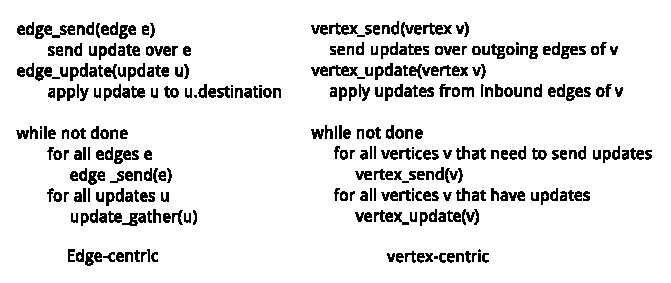
\includegraphics[width=0.6\textwidth]{myfigures/edgevertexcentric.eps}
\caption{以边为中心和以顶点为中心的算法流程}\label{fig:evc}
\vspace{\baselineskip}
\end{figure}



\section{并发技术}

随着计算机多核处理器的出现和内存不断增大,单台计算机的计算性能实际上已经有着很大的提升。
在过去40多年时间里,计算机性能一直遵循着摩尔定律,集成电路上可容纳的晶体管数目,约每隔18个月便会增加一倍,而集成电路的性能(计算能力)也将提升一倍。近年来,集成电路的集成程度已经非常高,芯片上元件的几何尺寸不可能无限制的缩小下去,摩尔定律面临挑战,遭遇瓶颈。另外,仅仅提高单核芯片的速度会产生过多的热量并且无法带来相应的性能改善。然而,人们对于电脑的要求不断提高,迫使处理器向高性能的方向发展。如果多一颗同一性能的处理器,理论上处理能力是原来的两倍。于是,为了进一步提高性能,就需要更多的处理器,将多个处理器置入单一芯片中,构成多核心处理器。于是,有相关学者和研究人员提出基于单机共享内存的图处理系统,例如GraphChi、X-Stream等。实验证明,这些单机上图处理系统经过严谨而合理的设计不仅具有高效便捷的优势,还能大大的降低开发成本。但是,随着网络的发展,数据量的海量递增趋势已经越来越明显,现有的一些单机系统在扩展性上很难满足这样的挑战。目前应用于企业级的图处理系统大部分仍然基于BSP模型的分布式系统,而现有单机系统往往从系统IO优化处着手,两者之间很难互相兼容。另外,局限于目前多核的并发编程理论并不成熟,造成单机环境下多核计算机的计算能力并没有被充分利用。传统上的单机多核并行软件开发往往是基于共享内存的,共享内存就很容易引起竞争条件,为保证程序的准确性和一致性,就必须对可能引起竞争的变量或者语句进行加锁保证互斥或者进行同步。此外,从硬件层面考虑,多核虽然提高了计算性能,但是随着核数的增多,核与核之间也会出现消息通讯,内存数据一致性等问题.

常见的图算法有遍历、最短路径、最大连通分量等。对于规模较小可以完全载入内存的图,单线程的处理方式需要顺序依次对顶点进行遍历访问即可。但是,当图的规模巨大时,这种单线程的执行方式就难以满足需求。大规模图的处理技术同时具有IO密集型和计算密集型两种特点。IO密集型是因为大规模图对象数据量庞大,无法一次性全部载入内存进行计算,同时还会涉及大量的中间结果的读写。而计算密集型则是因为基于大规模图对象的应用需要对整个图进行分析计算,涉及大量的迭代和计算。因此,传统的单线程的开发方式不仅能造成IO阻塞降低图处理的效率,还无法充分发挥多核计算机的有事,造成计算资源的浪费。因此,对于大规模图对象的处理一般采用并发的方式来提高图处理的效率。

为了能够更加有效的利用硬件所提供的性能,传统的应用开发方式现在已经不适用了。以往的应用开发方式在大部分情况下所面对的都是只有一个单独的处理器,也就是意味着顺序执行的单线程应用。如今,多核计算机逐渐成为主流配置,并且价格也在不断地降低。而要处分发挥多核计算机的计算能力,最简单的办法就是利用并发,编写能够在多个核心上运行的任务,并且任务之间可以通过共享数据的方式进行通信协同工作,也就是并发程序。


\subsection{大规模图处理中的并发技术}

大规模图对象因其数据量之庞大,传统的顺序的完全载入内存的方式不适合处理大规模图对象。如果需要将所有图都载入内存当中进行计算,就需要使用分布式的计算资源,将图分为若干部分,均衡的分配给每一个计算节点,同时不同的计算节点之间需要互相通讯以交换数据。

以顶点为中心的计算模型从概念上将顶点看做一个单独的执行单元。由于计算机的基本调度单位是线程,即使是把图均衡的分配在不同的计算节点上,也无法满足每个顶点同时并行执行,所以需要多线程并发技术来进一步提高图处理的效率。采用多线程的并发技术,可以将图按照一定的规则分配给不同的线程,每个线程负责一部分顶点。多线程下以顶点为中心的处理流程如下:
\begin{itemize}
\item 线程$T_0$读取顶点$s$。
\item 从磁盘读取顶点$s$的所有消息。
\item 调用用户自定义的消息处理函数,并更新该顶点的状态信息。
\item 线程$T_0$负责将消息放入自己的消息发送缓冲区,如果缓冲区已满,则将消息发送给顶点的邻接顶点。
\item 如果顶点$s$的邻接顶点位于同一个线程上,那么该线程就需要将消息进行缓存;如果位于不同的线程$T_i$上,那么就需要进行线程之间的消息通讯,将消息发送给该线程。线程$T_i$将线程保存在自己的阻塞消息队列中,等消息队列满的时候,然后根据消息的接受者的$id$,将所有消息进行缓存,并清空消息队列。
\end{itemize}

由于消息的接受者可能位于不同的线程,所以不同的线程之间需要大量的消息通讯,为了提高效率每个线程都有自己的消息发送缓存和消息接受缓存。此外,这些消息在下一个超级步来临之前并不会被处理,所以某个线程接收到消息之后,就需要将这些消息写入到磁盘上,所以一般而言每个线程同时会设置一个读写的缓冲区。多线程的并发技术提高了图计算过程中的数据吞吐量和处理效率。但是由于目前编写正确的并发程序依然非常困难,这是因为多线程并发往往是基于共享内存的,容易出现同步、阻塞和死锁\cite{srinivasan2006thread}。

\subsection{Actor并发模型}

虽然多线程的并发技术提高了图处理的数据吞吐量和处理效率,但是当线程的缓冲区被写满的时候需要引入大量而频繁的IO操作,所以会当前线程会挂起。多线程频繁的上下文切换依然是一个非常重量级的操作。另外,图计算不仅仅属于计算密集型,还属于IO密集型。尽管以顶点为中心的计算模型简化了大规模图处理的流程,但是多线程的并发技术还是引入了一定的复杂性。

Actor角色模型是一种不同于内存共享的并发技术。角色模型是用“角色”的概念,每个Actor角色都通过是用邮箱来异步的传递消息。角色模型中的语义概念非常贴近人们的实际生活中的概念,例如,邮箱类似于生活中的邮箱,消息发送到邮箱,人们可以从邮箱中获取邮件,类似的角色可以通过邮箱接受消息。在Actor角色模型中,主要的对象有三个:角色、邮箱和消息。角色是Actor并发模型中的执行运算的主体;邮箱则是角色接受消息的缓冲区;消息则是角色执行运算的驱动。角色的消息发送过程是异步,发往不同角色的消息不共享。消息一旦生成,一般不能被非接收Actor修改。角色之间可以并发执行,不必顺序执行。同时由于邮箱将不同的角色的在内存中的地址空间分开,不存在内存共享和同步的问题,所以在角色模型中没有锁和同步块的概念,也不会出现因为同步或者死锁而引发的问题。基于以上特点,角色模型能够支持更高并发量,角色之间的切换更加轻量级,也更加安全。

在JVM平台上,常见的Actor角色并发模型实现有Scala Actor、Jetlang、Akka和Kilim等。有学者\cite{karmani2009actor}对这些常见的Actor库,对各种库分别从状态封装性、安全的消息传递、调度等方面进行介绍和说明,如\ref{table:actors}所示。最后通过Threadring测试包对各个库进行并发度和消息分发速度等方面进行性能测试,结果表明Kilim拥有最好的效果。从以顶点为中心的计算模型的角度考虑,Actor并发模型比线程并发更加适合处理大规模图对象。Actor角色模型中,角色能够接受消息,执行计算,发送消息,从语义上非常接近顶点本身。可是,目前关于Actor并发模型在图计算中的应用并没有相关的工作,缺乏相关的可参考对比的标准。本文从探索性、简化问题的角度考虑,选择kilim作为本文的Actor并发模型。

\begin{table}[htbp]
\caption{JVM平台的Actor库}\label{table:actors}
\vspace{0.5em}\centering\wuhao
\begin{tabular}{|c|c|c|c|c|}
\toprule[1.5pt]
类库 & 封装性   & 公平调度   & 位置透明 & 移动性  \\
\midrule[1pt]
Scala Actor & 否 &是& 否 & 否\\
Kilim & 否 & 否 & 否 & 否\\
Actor Foundry & 是 & 是& 是 & 是\\
Jetlang & 是 & 否 & 是 &  否 \\
Akka &  是 & 是& 是 & 是\\
\bottomrule[1.5pt]
\end{tabular}
\vspace{\baselineskip}
\end{table}


\subsection{Kilim简介}

Kilim\cite{srinivasan2008kilim,srinivasan2010kilim,srinivasan2006thread}是一个使用原生JAVA编写的角色模型的并发库。在Kilim中,主要的角色模型用$Task$类表示,邮箱使用$Mailbox$类表示。Kilim的角色并发过程主要由一个称为Weaver的后期进程来实现,该进程需要直接修改类的字节码,从而使包含有$Pausable$签名的方法在运行时能够支持调度程序的快速调度。
Kilim不支持公平的调度,它的调度程序总是调度最需要对消息进行处理的角色运行。调度程序启动有限数量的内核线程。在有限的内核线程的基础上,启动更多的轻量级线程或者角色,即$Task$,每个$Task$的状态信息由$Fiber$类对其进行管理,不需要陷入内核线程,从而实现快速的上下文的切换和调度。

通过继承$Task$类可以实现一个角色,Kilim的$Mailbox$类提供了诸多的消息发送和接收消息。一般而言,一个角色需要一个邮箱,但是Kilim中角色和邮箱的实现是分离的,也就意味着,可以根据具体应用的不同而灵活的组合角色和邮箱,基于Kilim编写代码也很简单,只需要继承$Task$类,覆盖$execute$方法,并将相应的执行逻辑放在该方法内即可。然后通过如下三个步骤完成:

\begin{itemize}
\item  编译: javac -d ./classes 类名.java
\item weave:   java kilim.tools.Weave -d ./classes 类名全称
\item 运行:     java -cp ./classes:./classes:\$CLASSPATH  类名
\end{itemize}

\section{磁盘IO}
在大规模图处理中,除了需要将大量的数据到写入到磁盘中,同时图数据的访问又极易出现随机无序访问。在单机的图处理系统中,IO问题成为关注的重点,如何避免图数据的随机访问成为单机图处理系统提升效率的主要问题。目前,单机系统中针对IO的优化操作主要有两种:顺序访问和异步IO。

\subsection{顺序访问}
顺序访问就是按照数据存储的先后次序依次进行数据读写操作。采用顺序访问的好处在于不必把全部数据都载入内存中,只需要读取部分数据,处理部分数据即可。而在大规模图中,图的顶点之间的联系会非常的多,一条边可能一个顶点存在于内存,另一个顶点依旧保存在磁盘上,对顺序访问带来巨大的挑战。为达到顺序访问的目的,可以对边按照起始顶点进行排序,同时把边按照目的顶点进行分区,如此对分区依次进行访问,以后每次访问的数据总在当前数据访问位置的下方。
\subsection{异步IO}
异步IO的概念是相对于同步IO而言。在同步IO中,IO请求发出后,当前的执行过程会被阻塞直到IO操作完成返回结果之后,当前的执行过程才会继续执行。在大规模图处理过程中,会频繁的处理IO操作,同步IO会降低处理的效率。对于异步IO而言,异步调用过程发出之后,当前的执行过程会继续进行,并不会等待将消息写入磁盘完成,提高图计算的效率。

\subsection{内存映射}


内存映射是由操作系统提供的一种将文件映射到某一进程或者应用程序的地址空间的一种技术。该技术的主要目的就是为了提升对磁盘数据的访问效率。通过内存映射技术,进程或者应用程序就可以对文件进行随机访问。在32位的操作系统上,内存映射的大小有限,最大只能映射2GB的文件;在64位的操作系统中,通过内存映射技术可以映射非常巨大的文件。有学者\cite{yuhuibin2010neicunyingshe,yangningxue2004neicunyingshe}对内存映射在大数据处理上进行相关研究,事实证明内存映射不仅有助于快速处理数据同时还能节省大量额外的IO管理等操作。所以,对于单机上的大规模图处理而言,内存映射技术可以很好的解决图处理过程中的随机访问的问题。


\section{小结}

本章首先对图相关的概念和术语进行了介绍,并对图的相关常用算法进行说明;然后针对大规模图处理分别从计算模型、并发技术以及磁盘IO三个方面进行了详细的讨论和说明:在计算模型中,以Vertex-Centric模型作为介绍的中心,并且详细的说明为什么在Vertex-Centric之外需要BSP计算模型,同时与Edge-Centric模型进行了对比;接下来讨论多线程并发模型在在大规模图处理中的应用细节,同时指出存在于多线程并发技术中的复杂性,继而引入本文的并发技术Actor角色并发模型,并对本文选择的Actor并发库Kilim进行了简要的介绍;最后,从磁盘IO的角度对大规模图的处理进行相关的介绍与分析。